\documentclass{standalone}

\usepackage{tikz}

\begin{document}

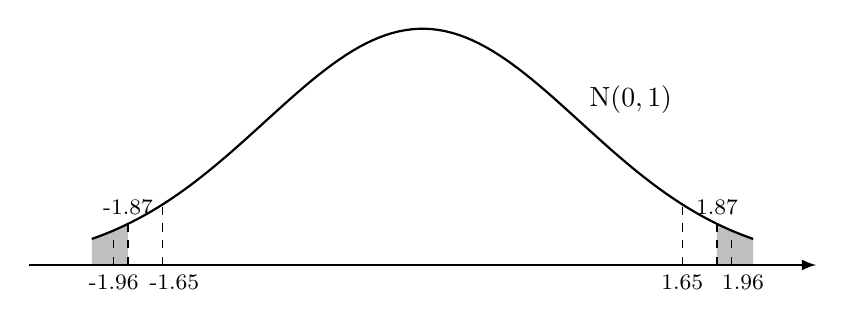
\begin{tikzpicture}[xscale=2, yscale=3]
    \fill[gray!50](-2.1, 0)--(-2.1, 0.11)--(-1.87, 0.174)--(-1.87,0);
    \fill[gray!50](2.1, 0)--(2.1, 0.11)--(1.87, 0.174)--(1.87,0);
    \draw[thick, -latex](-2.5, 0)--(2.5, 0);
    \draw[thick, domain=-2.1:2.1, samples=100]plot(\x,{exp(-\x*\x/2)});
    \node[above right]at(1, 0.6){$\mathrm{N}(0,1)$};
    \draw[dashed](1.65, 0)node[below]{\footnotesize 1.65}--(1.65, 0.256);
    \draw[dashed](1.87, 0)--(1.87, 0.174)node[above]{\footnotesize 1.87};
    \draw[dashed](1.96, 0)node[below]{\footnotesize\quad 1.96}--(1.96, 0.146);
    \draw[dashed](-1.65, 0)node[below]{\footnotesize\quad -1.65}--(-1.65, 0.256);
    \draw[dashed](-1.87, 0)--(-1.87, 0.174)node[above]{\footnotesize -1.87};
    \draw[dashed](-1.96, 0)node[below]{\footnotesize -1.96}--(-1.96, 0.146);
\end{tikzpicture}

\end{document}